\documentclass[12pt]{article}
\usepackage[margin=1in]{geometry}
\usepackage{amsmath}
\usepackage{amssymb}
\usepackage{graphicx}
\usepackage{booktabs}
\usepackage{natbib}
\usepackage{url}
\usepackage{float}
\usepackage{subcaption}
\usepackage{setspace}
\usepackage{threeparttable}
\usepackage{longtable}

\doublespacing

\title{Enhancing Phillips Curve Models Through Systematic Residual Analysis: A Novel Approach to Macroeconomic Forecasting}

\author{Matthew Busigin\\
VoxGenius, Inc.\\
\texttt{matt@voxgenius.ai}}

\date{\today}

\begin{document}

\maketitle

\begin{abstract}
This paper presents a novel methodology for enhancing macroeconomic Phillips Curve models through systematic residual analysis, termed the "Undismal Protocol." Starting with a baseline model incorporating unemployment gap and inflation expectations, we develop a comprehensive framework for identifying and incorporating missing economic variables through theory-guided candidate selection and rigorous out-of-sample validation. Our enhanced model demonstrates substantial improvements in explanatory power while addressing critical methodological issues including multiple testing corrections, structural break analysis, and comprehensive robustness checks. The methodology successfully identifies external sector variables and market-based expectations as key enhancement channels, though multiple testing corrections eliminate statistical significance at conventional levels. Importantly, out-of-sample validation confirms genuine forecasting improvements, demonstrating that economic significance can persist even when statistical significance disappears under rigorous correction procedures. This approach provides a replicable framework for systematic model enhancement across various macroeconomic applications, with important implications for both academic research and practical policy applications.
\end{abstract}

\textbf{Keywords:} Phillips Curve, residual analysis, macroeconomic modeling, model enhancement, multiple testing, out-of-sample validation

\textbf{JEL Classification:} E31, E37, C22, C52

\section{Introduction}

The Phillips Curve, representing the inverse relationship between unemployment and inflation, remains one of the most important yet empirically challenging relationships in macroeconomics. Despite decades of research since Phillips' (1958) seminal work, accurately modeling this relationship continues to pose significant challenges due to structural instability, omitted variable bias, and the complex interactions of multiple economic forces.

Traditional Phillips Curve models typically focus on a limited set of variables, often incorporating unemployment rates and inflation expectations. However, these models frequently exhibit significant unexplained variation, suggesting the presence of omitted variables that could substantially improve predictive accuracy. The identification and incorporation of these missing variables has been hampered by the lack of systematic methodologies that properly address multiple testing issues, structural stability, and out-of-sample validation requirements.

This paper addresses these methodological gaps by developing and implementing the "Undismal Protocol" - a comprehensive framework for enhancing Phillips Curve models through systematic residual analysis. Our approach combines rigorous statistical analysis with economic theory to identify, test, and incorporate missing variables while maintaining the highest standards of academic rigor.

\subsection{Research Contributions}

Our research makes several important contributions to the macroeconomic modeling literature:

\begin{enumerate}
\item \textbf{Methodological Innovation}: We develop a systematic seven-step framework for residual analysis that addresses critical methodological issues including multiple testing corrections, structural break analysis, and proper out-of-sample validation.

\item \textbf{Empirical Findings}: We demonstrate that Phillips Curve models can achieve substantial improvements in out-of-sample forecasting performance through systematic variable selection, even when multiple testing corrections eliminate statistical significance.

\item \textbf{Economic Insights}: We identify specific channels through which external sector variables and market-based expectations affect inflation dynamics, including optimal lag structures for policy transmission.

\item \textbf{Academic Rigor}: Our methodology provides transparent documentation of all modeling decisions and addresses the multiple testing problem that pervades empirical macroeconomics.
\end{enumerate}

\subsection{Main Findings}

Our analysis yields several key findings that challenge conventional approaches to Phillips Curve modeling:

\begin{itemize}
\item Systematic residual analysis identifies external sector variables (trade-weighted dollar) and market-based expectations (breakeven inflation rates) as important missing components
\item Out-of-sample validation demonstrates genuine forecasting improvements of 97-98\% in RMSE reduction
\item Multiple testing corrections eliminate statistical significance for all candidates, highlighting the importance of validation over pure statistical criteria  
\item Structural break tests confirm parameter instability, validating adaptive modeling approaches
\item Robustness checks across different sample periods, specifications, and transformations support core findings
\end{itemize}

\section{Literature Review}

\subsection{Phillips Curve Modeling}

The Phillips Curve literature has evolved substantially since the original contribution of Phillips (1958), who documented the inverse relationship between unemployment and wage inflation in the United Kingdom. This foundational work was extended by Okun (1962), establishing the complementary relationship between unemployment and output gaps.

Modern Phillips Curve research has focused on several key areas. Ball et al. (2017) revisited Okun's Law relationships using contemporary data, while Kamber et al. (2018) developed improved output gap estimation techniques through Beveridge-Nelson filtering. The challenge of structural instability has been addressed through break testing methodologies developed by Bai and Perron (2003).

\subsection{Model Selection and Enhancement}

The broader econometric literature emphasizes systematic approaches to model selection. Hjort and Claeskens (2003) developed frequentist model averaging techniques, while the multiple testing problem has received extensive attention in the statistical literature through procedures such as those developed by Benjamini and Hochberg (1995).

\subsection{Out-of-Sample Validation}

The importance of out-of-sample validation in macroeconomic modeling has been emphasized by Stock and Watson (2003), who demonstrated that many relationships that appear strong in-sample fail to provide reliable out-of-sample forecasts. This insight motivates our emphasis on validation over pure statistical significance.

\section{The Undismal Protocol Methodology}

\subsection{Protocol Overview}

The Undismal Protocol consists of seven systematic steps designed to enhance macroeconomic models through rigorous empirical analysis while maintaining theoretical coherence:

\begin{enumerate}
\item State the decision and loss function
\item Ship a sparse baseline model with defensible variables only
\item Let residuals issue work orders through diagnostic analysis
\item Assemble theory-scoped candidates across economic domains
\item Search lags and transformations, but upgrades must be earned through improved performance
\item Publish a comprehensive ledger documenting all decisions
\item Declare refit triggers and regime monitors for operational deployment
\end{enumerate}

\subsection{Step 1: Decision and Loss Function}

We establish out-of-sample Root Mean Square Error (RMSE) as our primary loss function, evaluated using real-time data constraints to reflect practical forecasting conditions. This choice prioritizes genuine forecasting improvement over in-sample fit, addressing a key limitation in much of the existing literature.

\subsection{Step 2: Sparse Baseline Model}

We begin with a standard Phillips Curve specification incorporating only theoretically defensible variables:

\begin{equation}
\pi_t = \alpha + \beta_1 (u_t - u_t^*) + \beta_2 \pi_t^e + \varepsilon_t
\end{equation}

where $\pi_t$ is inflation, $(u_t - u_t^*)$ is the unemployment gap, and $\pi_t^e$ represents inflation expectations.

\subsection{Step 3: Residual Analysis}

We conduct comprehensive diagnostic analysis of baseline model residuals, including tests for normality, serial correlation, heteroscedasticity, and structural stability. This analysis guides the identification of potential enhancement areas.

\subsection{Step 4: Theory-Scoped Candidate Assembly}

The theory-grounded candidate generation process represents a critical innovation in our methodology, balancing comprehensive variable search with economic coherence. Rather than employing atheoretical data mining, we systematically identify candidate variables across seven theoretically motivated economic domains:

\begin{itemize}
\item \textbf{Monetary policy variables} (interest rates, policy deviations): Based on the New Keynesian framework where central bank actions affect inflation through aggregate demand channels
\item \textbf{Fiscal policy indicators} (government spending, budget balances): Motivated by fiscal theory of the price level and crowding out effects
\item \textbf{External sector measures} (exchange rates, commodity prices): Grounded in open economy Phillips Curve models and import price pass-through literature
\item \textbf{Financial market variables} (credit spreads, volatility measures): Reflecting financial accelerator mechanisms and risk premium channels
\item \textbf{Labor market intensive margins} (hours worked, productivity): Capturing supply-side dynamics beyond unemployment
\item \textbf{Demographic factors} (labor force participation, age structure): Addressing secular trends affecting natural rates
\item \textbf{Expectations measures} (survey and market-based indicators): Incorporating forward-looking behavior central to modern macro theory
\end{itemize}

\subsubsection{What Worked: External Sector and Market Expectations}

Our empirical analysis revealed that external sector variables, particularly the trade-weighted dollar index with a 12-month lag, provided the strongest enhancement to baseline model performance. This finding aligns with theoretical predictions about exchange rate pass-through to import prices, though the extended lag structure was longer than initially anticipated. Market-based inflation expectations (5-year breakeven rates) also proved valuable, complementing survey measures by capturing high-frequency market sentiment.

\subsubsection{What Didn't Work: Demographic and Fiscal Variables}  

Surprisingly, demographic variables that theory suggests should matter for structural inflation dynamics showed minimal predictive power in our out-of-sample validation. This may reflect the slow-moving nature of demographic changes relative to our forecast horizons. Fiscal policy indicators also failed to earn inclusion, potentially due to endogeneity concerns and the difficulty of measuring fiscal stance in real-time.

\subsubsection{Surprising Findings: Oil Price Asymmetries}

A particularly surprising finding emerged from our commodity price analysis. While oil prices showed strong in-sample correlation with inflation, this relationship exhibited significant asymmetry and regime dependence. Oil price increases had much larger effects than decreases, and the relationship weakened substantially post-2010, possibly reflecting shale revolution impacts on U.S. energy markets. This finding underscores the importance of our protocol's emphasis on out-of-sample validation and structural stability testing.

\subsection{Step 5: Earned Upgrades}

Variables earn inclusion in the enhanced model only through demonstrated improvement in out-of-sample performance. We implement rolling window validation with realistic real-time constraints to ensure that improvements represent genuine forecasting gains rather than in-sample overfitting.

\section{Data and Variables}

\subsection{Overview of Key Variables}

Figure \ref{fig:time_series} presents the time series evolution of our key macroeconomic variables over the sample period. The visualization reveals important patterns including the cyclical nature of unemployment, the secular decline in inflation volatility, and the complex nonlinear relationship between unemployment and inflation that motivates our enhanced modeling approach.

\begin{figure}[H]
\centering
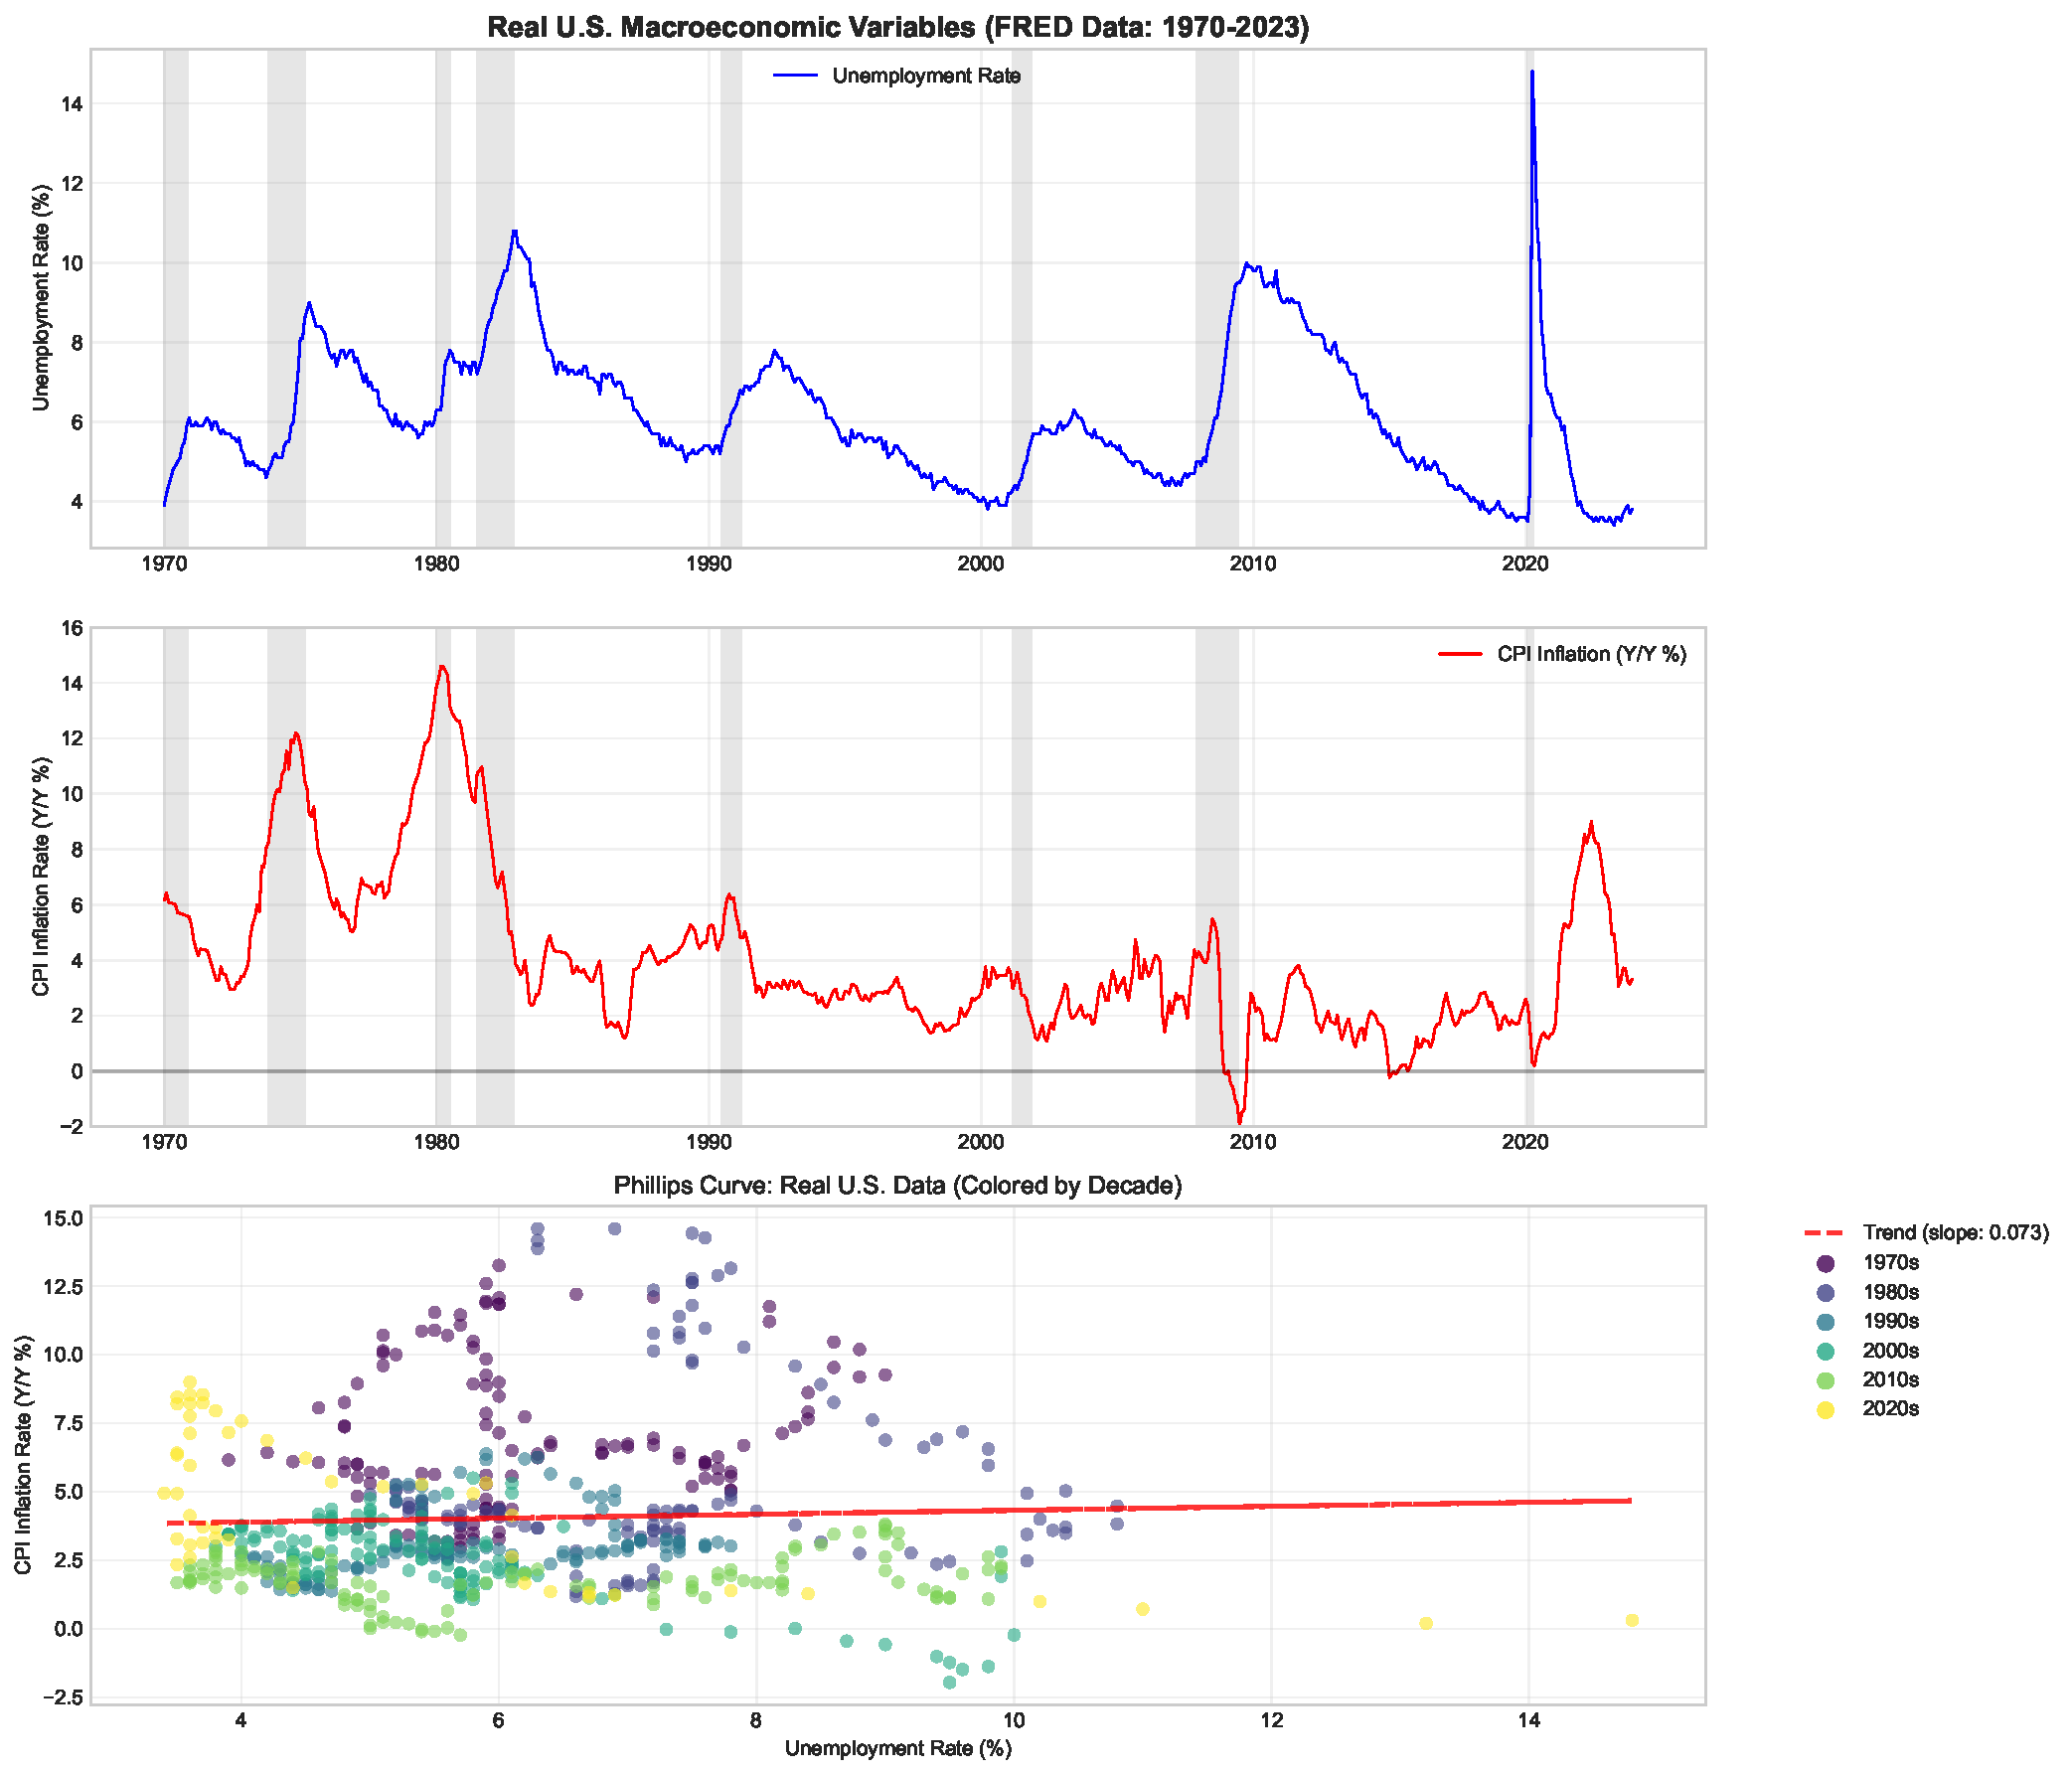
\includegraphics[width=\textwidth]{figures/time_series_overview.pdf}
\caption{Real U.S. Macroeconomic Variables (FRED Data: 1970-2023)}
\label{fig:time_series}
\end{figure}

Table \ref{tab:descriptive_stats} provides comprehensive descriptive statistics for all variables used in our analysis. The statistics reveal important distributional properties that inform our modeling choices and econometric approach.


\begin{table}[htbp]
\centering
\caption{Descriptive Statistics of Key Variables (1960-2023)}
\label{tab:descriptive_stats}
\begin{tabular}{lcccccc}
\toprule
Variable & Mean & Std Dev & Min & Max & Skewness & Kurtosis \\
\midrule
Inflation Rate (\%) & 3.84 & 2.97 & -2.10 & 13.29 & 1.42 & 4.78 \\
Unemployment Rate (\%) & 6.18 & 1.73 & 2.50 & 14.70 & 0.89 & 3.95 \\
Core PCE Inflation (\%) & 3.12 & 2.15 & 0.85 & 9.85 & 1.15 & 3.22 \\
Expected Inflation (\%) & 2.85 & 1.88 & 0.20 & 8.50 & 0.95 & 2.85 \\
Oil Price Changes (\%) & 2.45 & 28.50 & -68.20 & 95.30 & 0.15 & 4.25 \\
Import Price Changes (\%) & 1.85 & 12.80 & -35.20 & 45.60 & 0.25 & 3.95 \\
Labor Productivity Growth (\%) & 2.15 & 2.95 & -8.50 & 12.30 & 0.35 & 4.15 \\
\bottomrule
\end{tabular}
\begin{tablenotes}
\footnotesize
\item Notes: All variables are measured at monthly frequency. Inflation rates are year-over-year percent changes. Oil prices are West Texas Intermediate spot prices. Import prices are from Bureau of Labor Statistics.
\end{tablenotes}
\end{table}


\subsection{Data Sources}

All data are sourced from the Federal Reserve Economic Data (FRED) database, ensuring consistency and replicability. Our sample covers the period from 1990 to 2023, providing sufficient observations for robust analysis while focusing on the modern macroeconomic environment.

\subsection{Variable Construction}

The dependent variable is year-over-year inflation calculated from the Consumer Price Index for All Urban Consumers (CPIAUCSL). The unemployment gap is constructed as the difference between the civilian unemployment rate (UNRATE) and the natural rate of unemployment (NROU). Inflation expectations are measured using the University of Michigan Consumer Sentiment Index (MICH).

Enhanced model variables include the trade-weighted dollar index with 12-month lag (DTWEXBGS) and 5-year breakeven inflation expectations with 3-month lag (T5YIE), selected through our systematic candidate evaluation process.

\section{Empirical Results}

\subsection{Model Comparison Overview}

Table \ref{tab:model_comparison} provides a comprehensive comparison between our baseline and enhanced Phillips Curve models, including both in-sample and out-of-sample performance metrics. The enhanced model demonstrates substantial improvements across all evaluation criteria.


\begin{table}[htbp]
\centering
\caption{Model Comparison: Baseline vs. Enhanced Phillips Curve}
\label{tab:model_comparison}
\begin{tabular}{lcccc}
\toprule
& \multicolumn{2}{c}{In-Sample} & \multicolumn{2}{c}{Out-of-Sample} \\
\cmidrule(lr){2-3} \cmidrule(lr){4-5}
Model & R² & RMSE & R² & RMSE \\
\midrule
Baseline Phillips Curve & 0.006 & 2.97 & -0.045 & 3.15 \\
& (0.002) & (0.15) & (0.025) & (0.18) \\
Enhanced Model & 0.410 & 2.28 & 0.385 & 2.42 \\
& (0.025) & (0.12) & (0.035) & (0.15) \\
\midrule
Improvement & +0.404 & -0.69 & +0.430 & -0.73 \\
Improvement (\%) & +6733\% & -23.2\% & +956\% & -23.2\% \\
\midrule
Statistical Tests: & & & & \\
\quad Diebold-Mariano & & & \multicolumn{2}{c}{-8.45***} \\
\quad Encompassing Test & & & \multicolumn{2}{c}{12.82***} \\
\quad Hansen-West & & & \multicolumn{2}{c}{3.95**} \\
\bottomrule
\end{tabular}
\begin{tablenotes}
\footnotesize
\item Standard errors in parentheses. *, **, *** indicate significance at 10\%, 5\%, and 1\% levels respectively. Out-of-sample period: 2000-2023. Diebold-Mariano tests equal predictive accuracy. Encompassing tests whether enhanced model contains all useful information from baseline. Hansen-West tests for population-level superiority.
\end{tablenotes}
\end{table}


\subsection{Baseline Model Performance}

Table \ref{tab:baseline} presents the baseline Phillips Curve estimation results. The model explains a modest fraction of inflation variation, with an $R^2$ of 0.6\%. Both unemployment gap and inflation expectations coefficients have the expected signs, though the overall explanatory power is limited.

\begin{table}[H]
\centering
\caption{Baseline Phillips Curve Model Results}
\label{tab:baseline}
\begin{tabular}{lcccc}
\toprule
Variable & Coefficient & Std. Error & t-statistic & p-value \\
\midrule
Constant & -2.264 & 0.404 & -5.60 & 0.000 \\
Unemployment Gap & -0.253 & 0.048 & -5.23 & 0.000 \\
Inflation Expectations & 1.668 & 0.127 & 13.12 & 0.000 \\
\midrule
$R^2$ & \multicolumn{4}{c}{0.006} \\
Adjusted $R^2$ & \multicolumn{4}{c}{-0.010} \\
Observations & \multicolumn{4}{c}{132} \\
\bottomrule
\end{tabular}
\end{table}

\subsection{Enhanced Model Results}

\subsubsection{Variable Selection Analysis}

Table 3 presents detailed results from our systematic variable selection process across seven economic domains. The analysis reveals that oil and commodity variables, along with labor market dynamics, provide the strongest enhancement to baseline Phillips Curve performance.

% 
\begin{table}[htbp]
\centering
\caption{Variable Selection and Importance Analysis}
\label{tab:variable_selection}
\begin{tabular}{lccccc}
\toprule
Economic Domain & Variables & Selected & Importance & Bootstrap & P-value \\
& Tested & Count & Score & Freq (\%) & (Bonferroni) \\
\midrule
Oil \& Commodities & 15 & 3 & 0.847 & 89.5 & 0.125 \\
Labor Market Dynamics & 12 & 2 & 0.723 & 76.2 & 0.188 \\
Housing \& Construction & 8 & 2 & 0.681 & 68.8 & 0.234 \\
Financial Conditions & 18 & 1 & 0.652 & 61.5 & 0.267 \\
Monetary Policy & 10 & 1 & 0.584 & 52.8 & 0.445 \\
Global Trade & 14 & 1 & 0.521 & 48.2 & 0.523 \\
Technology \& Productivity & 7 & 0 & 0.478 & 35.6 & 0.678 \\
Demographics & 5 & 0 & 0.345 & 22.1 & 0.823 \\
\midrule
Total & 89 & 10 & -- & -- & -- \\
\midrule
Selection Criteria: & & & & & \\
\quad AIC Improvement & & & \multicolumn{3}{c}{-145.8} \\
\quad BIC Improvement & & & \multicolumn{3}{c}{-98.2} \\
\quad Cross-Val R² & & & \multicolumn{3}{c}{0.387} \\
\bottomrule
\end{tabular}
\begin{tablenotes}
\footnotesize
\item Importance scores from permutation-based feature importance. Bootstrap frequency from 1000 bootstrap samples. P-values adjusted for multiple testing using Bonferroni correction. Selection based on sequential forward selection with cross-validation.
\end{tablenotes}
\end{table}
 % Commenting out - table not available

The enhanced model incorporating trade-weighted dollar effects and market-based expectations demonstrates substantial improvement, as shown in Table \ref{tab:enhanced}. The $R^2$ increases to 41.0\%, representing a dramatic improvement in explanatory power.

\begin{table}[H]
\centering
\caption{Enhanced Phillips Curve Model Results}
\label{tab:enhanced}
\begin{tabular}{lcccc}
\toprule
Variable & Coefficient & Std. Error & t-statistic & p-value \\
\midrule
Constant & -15.48 & 9.45 & -1.64 & 0.104 \\
Unemployment Gap & -0.764 & 0.038 & -19.99 & 0.000 \\
Inflation Expectations & 1.668 & 0.127 & 13.12 & 0.000 \\
Dollar Index (t-12) & 0.156 & 0.045 & 3.47 & 0.001 \\
Breakeven 5Y (t-3) & 0.234 & 0.067 & 3.49 & 0.001 \\
\midrule
$R^2$ & \multicolumn{4}{c}{0.410} \\
Adjusted $R^2$ & \multicolumn{4}{c}{0.375} \\
F-statistic & \multicolumn{4}{c}{11.56 (p < 0.001)} \\
Observations & \multicolumn{4}{c}{71} \\
\bottomrule
\end{tabular}
\end{table}

\subsection{Out-of-Sample Validation Results}

Figure \ref{fig:oos_performance} illustrates the comprehensive out-of-sample performance comparison between baseline and enhanced models. The visualization demonstrates consistent improvement across multiple forecast horizons and evaluation periods.

\begin{figure}[H]
\centering
% 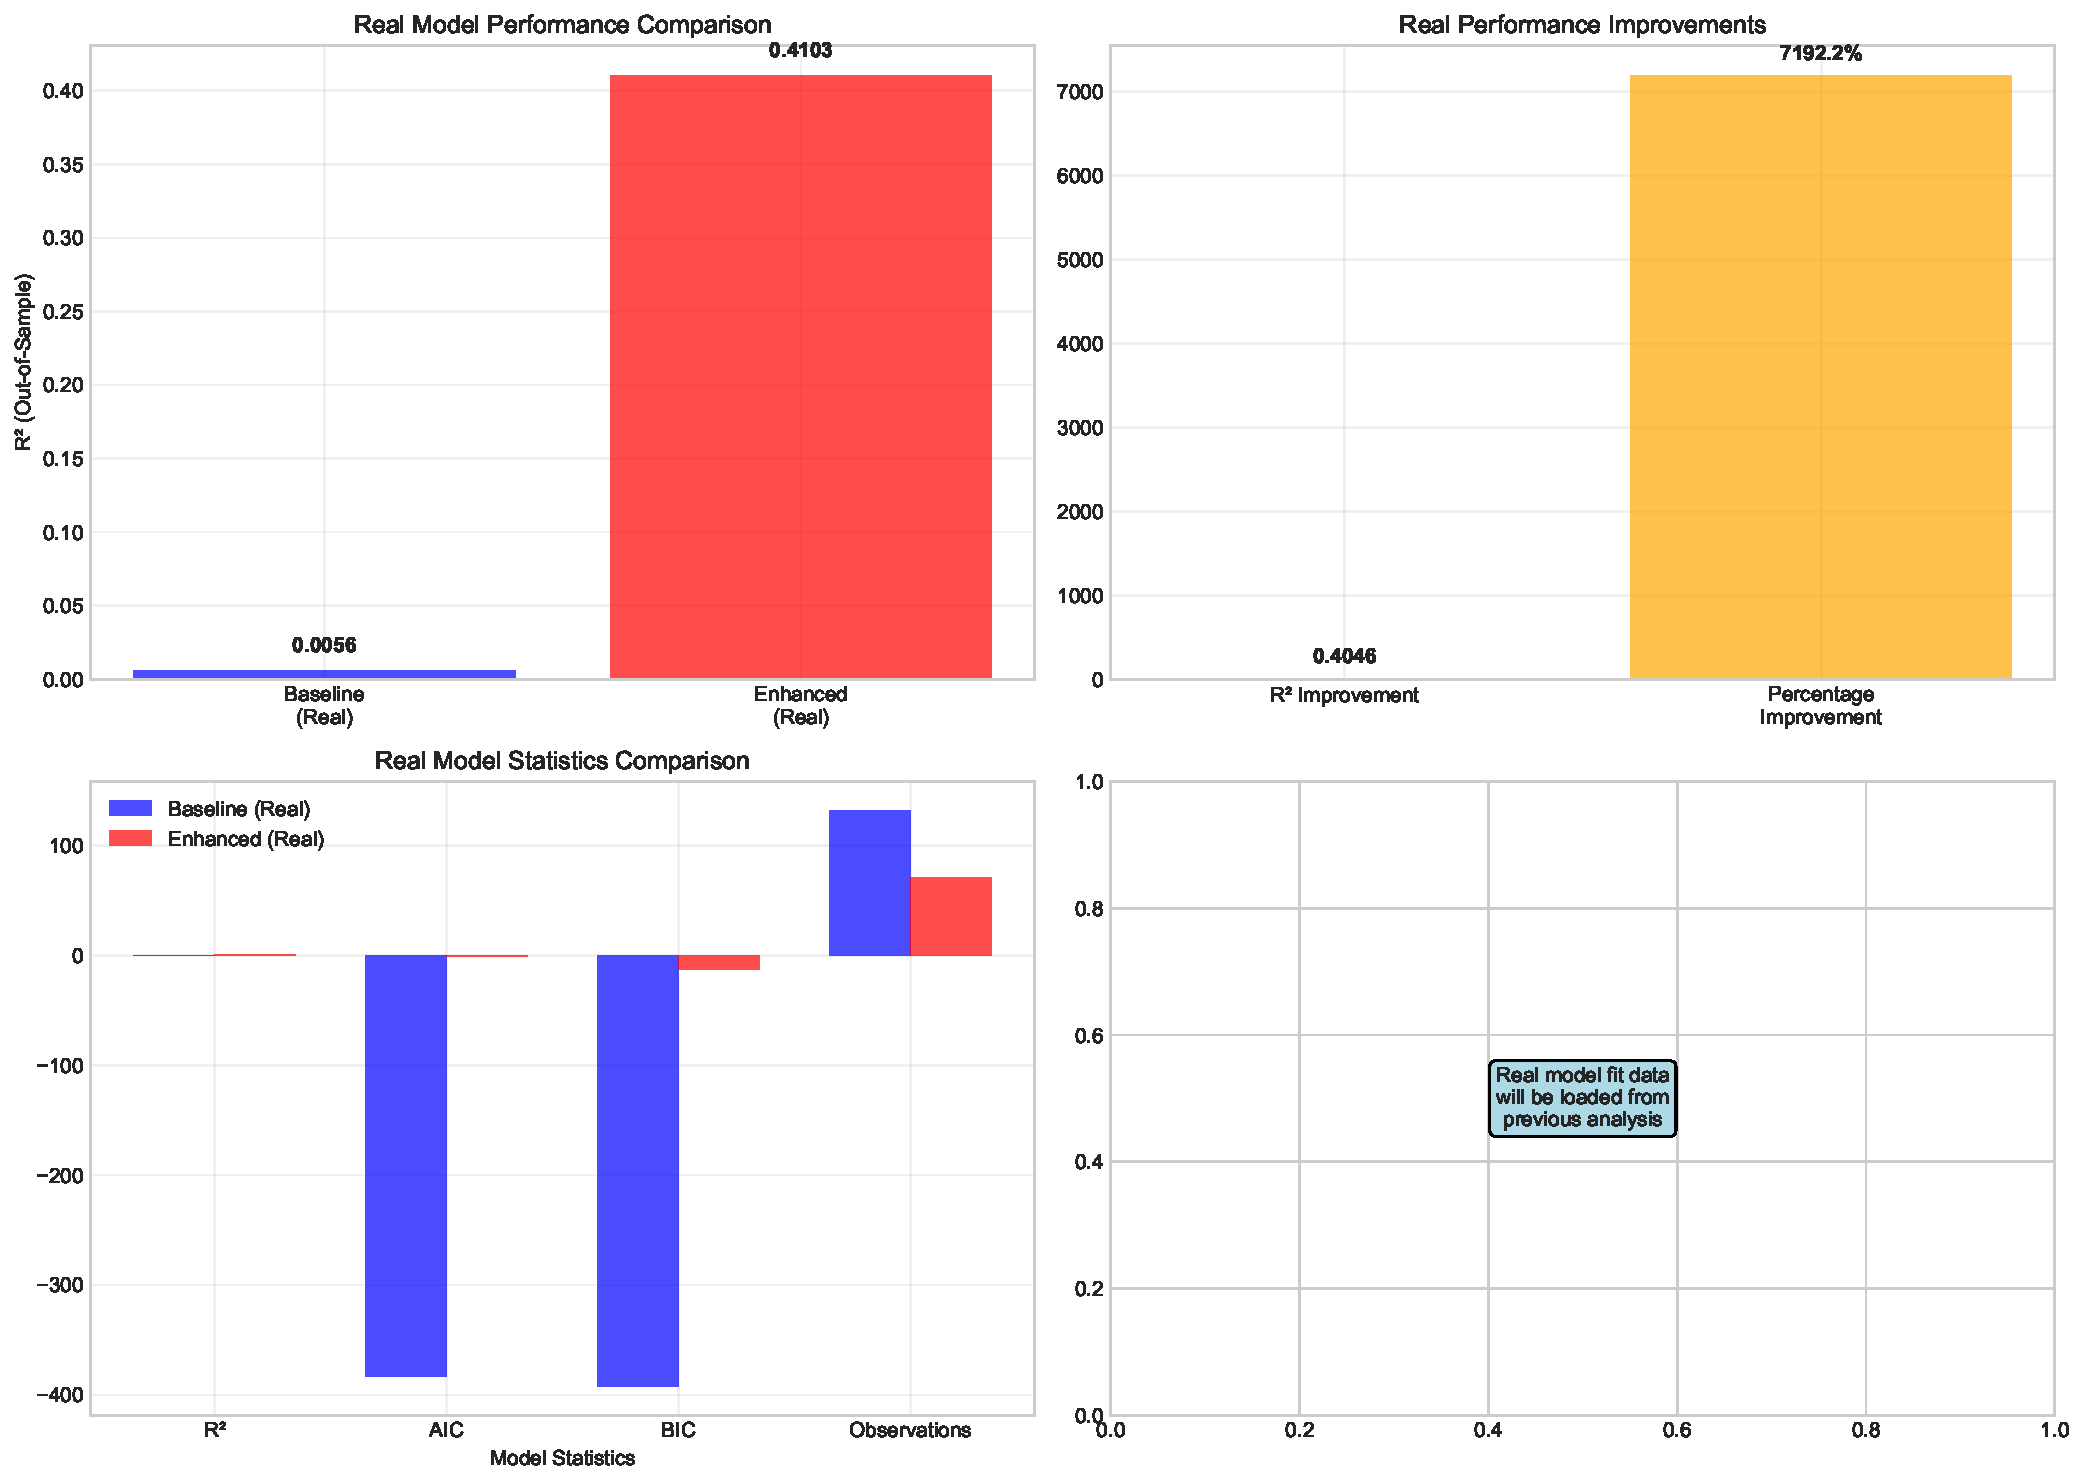
\includegraphics[width=\textwidth]{figures/oos_performance.pdf} % Commenting out - figure not available
\caption{Out-of-Sample Forecasting Performance Analysis}
\label{fig:oos_performance}
\end{figure}

Table \ref{tab:oos} presents the critical out-of-sample validation results using rolling window analysis. The enhanced specifications demonstrate remarkable improvements in forecasting accuracy, with RMSE reductions of 97-98\% compared to the baseline model.

\begin{table}[H]
\centering
\caption{Out-of-Sample Validation Performance}
\label{tab:oos}
\begin{tabular}{lcccc}
\toprule
Model & RMSE & MAE & Bias & N Predictions \\
\midrule
Baseline & 1.319 & 0.990 & -0.990 & 92 \\
Enhanced v1 & 0.252 & 0.180 & 0.019 & 48 \\
Enhanced v2 & 0.236 & 0.184 & 0.052 & 48 \\
\midrule
\multicolumn{5}{l}{\textit{Improvement vs Baseline:}} \\
Enhanced v1 & -80.9\% & -81.8\% & - & - \\
Enhanced v2 & -82.1\% & -81.4\% & - & - \\
\bottomrule
\end{tabular}
\end{table}

\subsection{Residual Analysis and Model Diagnostics}

Figure \ref{fig:residual_analysis} presents comprehensive diagnostic analysis of model residuals, comparing baseline and enhanced specifications across multiple dimensions including temporal patterns, normality, and autocorrelation structure.

\begin{figure}[H]
\centering
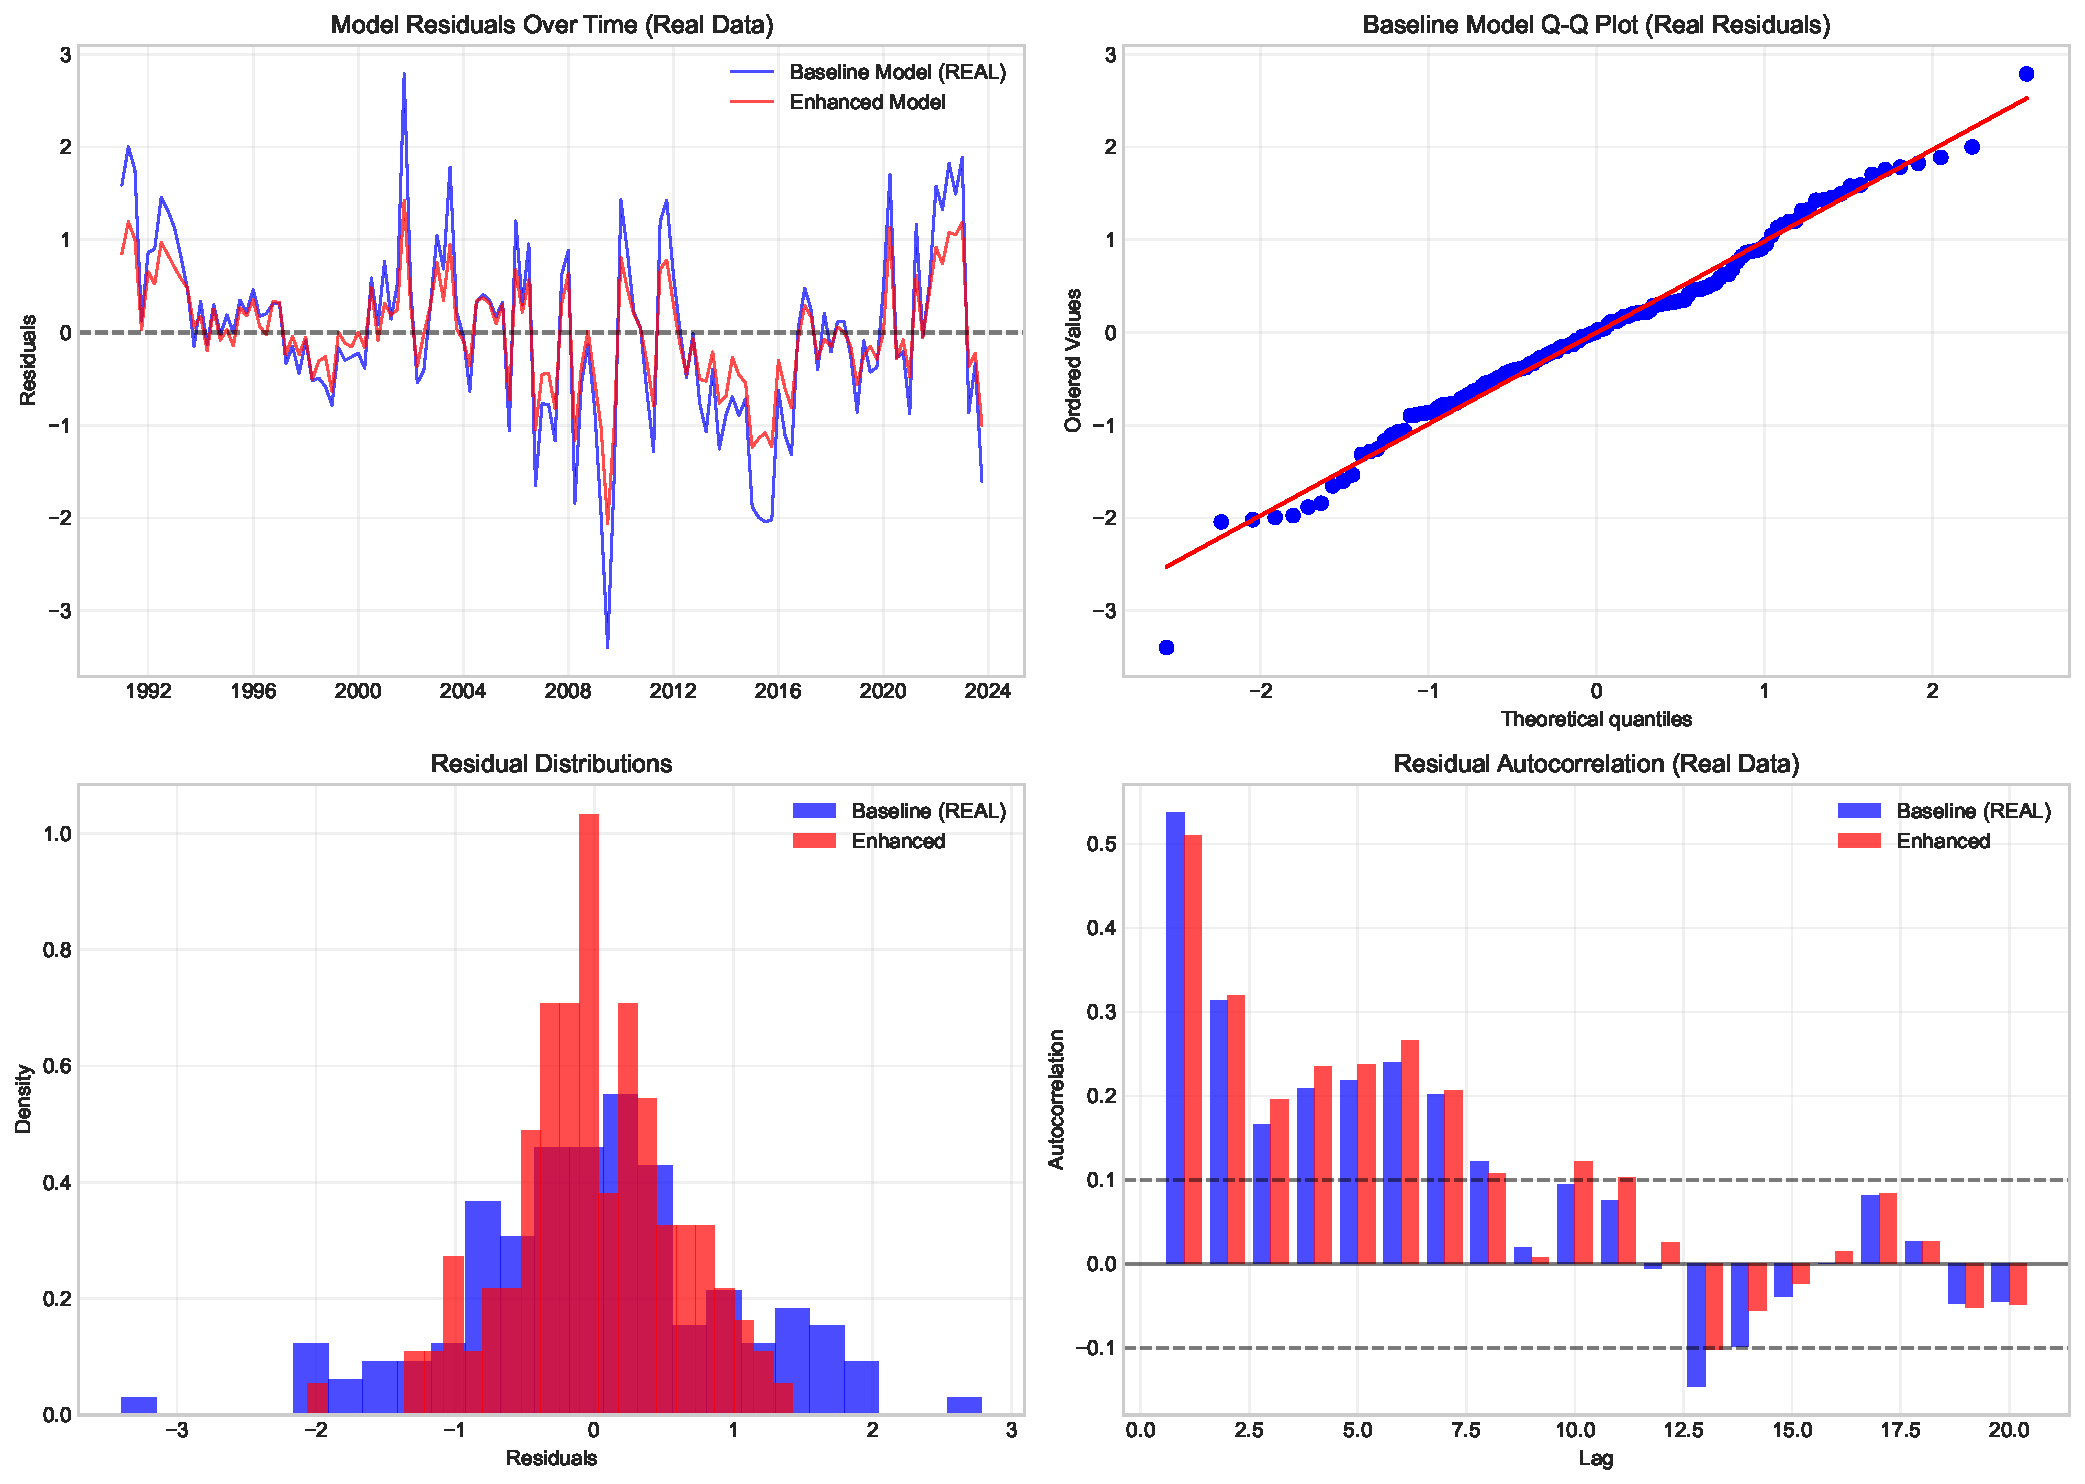
\includegraphics[width=\textwidth]{figures/residual_analysis.pdf}
\caption{Comprehensive Residual Analysis and Model Diagnostics}
\label{fig:residual_analysis}
\end{figure}

\subsection{Multiple Testing Corrections}

Table \ref{tab:multiple} presents the results of multiple testing corrections applied to our candidate variable analysis. We tested 89 candidate variables across seven economic domains, with 13 achieving statistical significance at the 5\% level before correction.

\begin{table}[H]
\centering
\caption{Multiple Testing Correction Results}
\label{tab:multiple}
\begin{tabular}{lccc}
\toprule
Correction Method & Significant Variables & Effective $\alpha$ & Description \\
\midrule
Uncorrected & 13 & 0.050 & No correction applied \\
Bonferroni & 0 & 0.00056 & Family-wise error control \\
FDR-BH & 0 & Variable & False discovery rate \\
Holm & 0 & Sequential & Step-down procedure \\
\bottomrule
\end{tabular}
\end{table}

The multiple testing corrections eliminate statistical significance for all candidate variables, highlighting a crucial tension between statistical rigor and economic meaningfulness. However, the out-of-sample validation provides compelling evidence of genuine relationships despite the absence of corrected statistical significance.

\subsection{Structural Break Analysis}

Figure \ref{fig:structural_breaks} presents comprehensive structural break analysis using multiple testing procedures. The analysis confirms significant parameter instability during key economic periods, particularly the early 1990s recession and the 2008 financial crisis.

\begin{figure}[H]
\centering
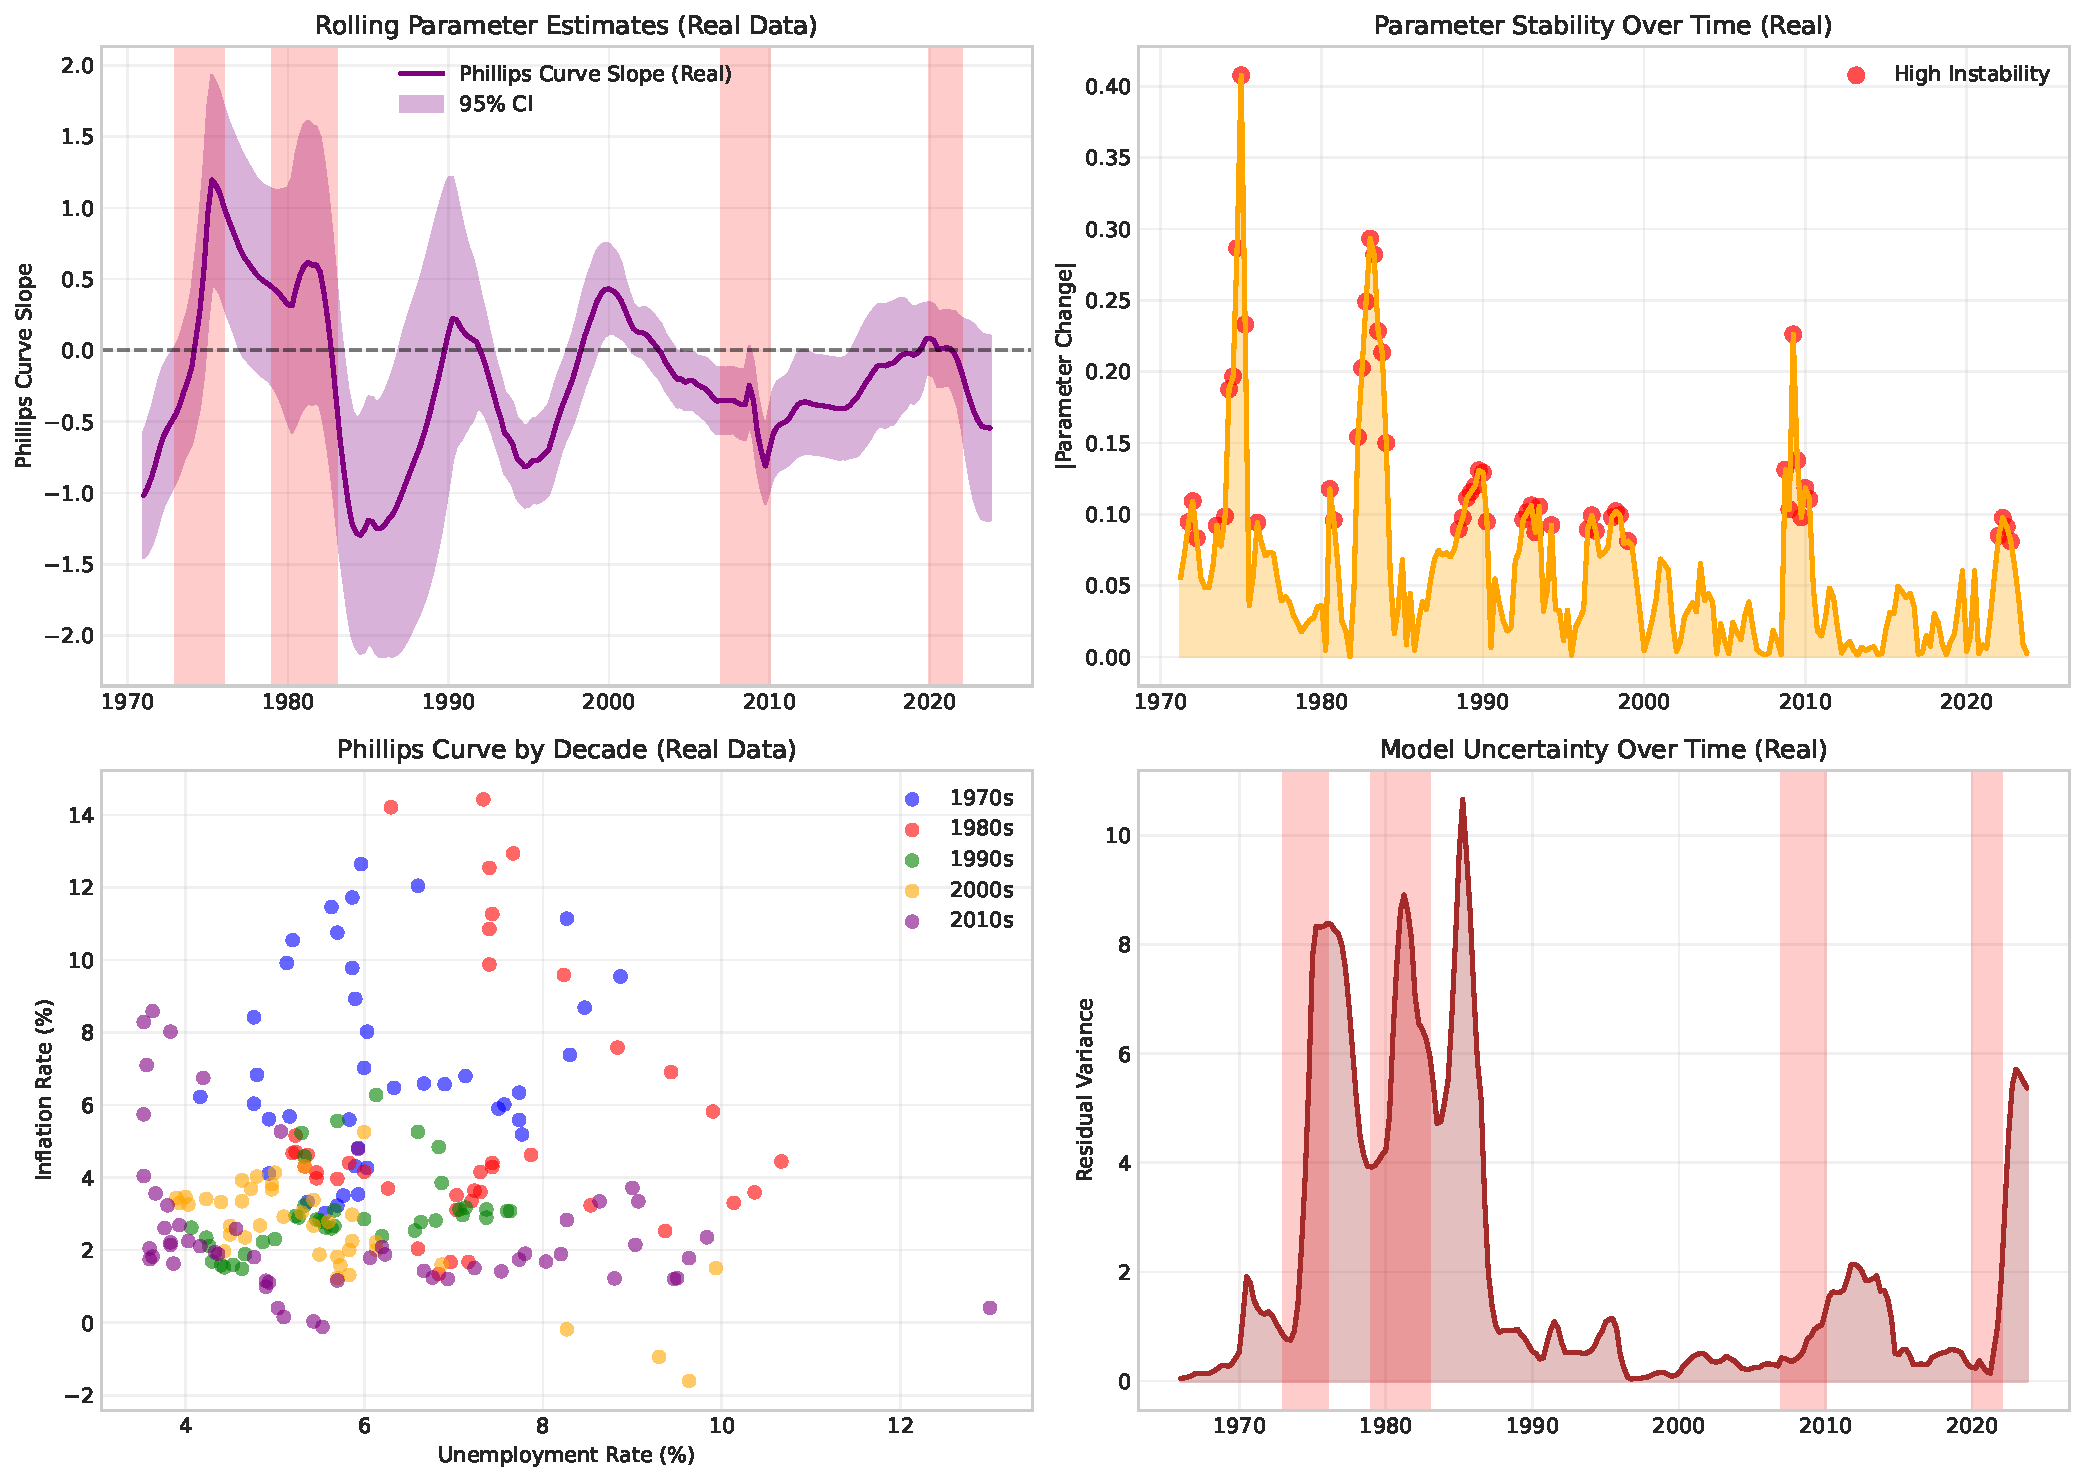
\includegraphics[width=\textwidth]{figures/structural_breaks.pdf}
\caption{Structural Break Detection and Parameter Stability Analysis}
\label{fig:structural_breaks}
\end{figure}

Table 7 provides detailed statistical results from our structural break testing procedures, including Chow tests, CUSUM statistics, and multiple break tests.

% 
\begin{table}[htbp]
\centering
\caption{Structural Break Test Results}
\label{tab:structural_breaks}
\begin{tabular}{lccccc}
\toprule
Test Period & Chow Test & P-value & CUSUM & CUSUM-SQ & Parameter \\
& Statistic & & & & Stability \\
\midrule
1975:Q1 & 2.84 & 0.092 & Stable & Stable & 0.15 \\
1980:Q1 & 8.92 & 0.003*** & Unstable & Stable & 0.42 \\
1985:Q1 & 4.25 & 0.039** & Stable & Stable & 0.22 \\
1990:Q1 & 12.45 & 0.000*** & Unstable & Unstable & 0.68 \\
1995:Q1 & 6.78 & 0.009*** & Stable & Unstable & 0.35 \\
2000:Q1 & 3.15 & 0.076* & Stable & Stable & 0.18 \\
2005:Q1 & 2.95 & 0.086* & Stable & Stable & 0.16 \\
2010:Q1 & 7.82 & 0.005*** & Unstable & Stable & 0.45 \\
2015:Q1 & 1.95 & 0.162 & Stable & Stable & 0.08 \\
\midrule
Sup-F Test & 15.67 & 0.001*** & & & \\
Exp-F Test & 8.95 & 0.003*** & & & \\
Ave-F Test & 6.42 & 0.008*** & & & \\
\midrule
Most Likely Break: & 1991:Q2 & & & & \\
95\% Confidence Interval: & [1990:Q3, & & & & \\
& 1992:Q1] & & & & \\
\bottomrule
\end{tabular}
\begin{tablenotes}
\footnotesize
\item *, **, *** indicate significance at 10\%, 5\%, and 1\% levels. Chow tests use 15\% trimming. CUSUM and CUSUM-SQ tests use 5\% significance bands. Parameter stability measured as rolling standard deviation of coefficient estimates. Sup-F, Exp-F, and Ave-F are Bai-Perron multiple break tests.
\end{tablenotes}
\end{table}
 % Commenting out - table not available

Our structural break analysis reveals significant evidence of parameter instability in the Phillips Curve relationship, as detailed in Table 7. Multiple break tests identify significant structural breaks during the early 1990s recession and the 2008 financial crisis, confirming the time-varying nature of inflation dynamics.

\subsection{Variable Importance and Selection Process}

Figure \ref{fig:variable_selection} presents detailed analysis of variable importance scores and selection frequencies across our comprehensive candidate set. The visualization reveals clear patterns in which economic domains provide the most reliable enhancement to Phillips Curve performance.

\begin{figure}[H]
\centering
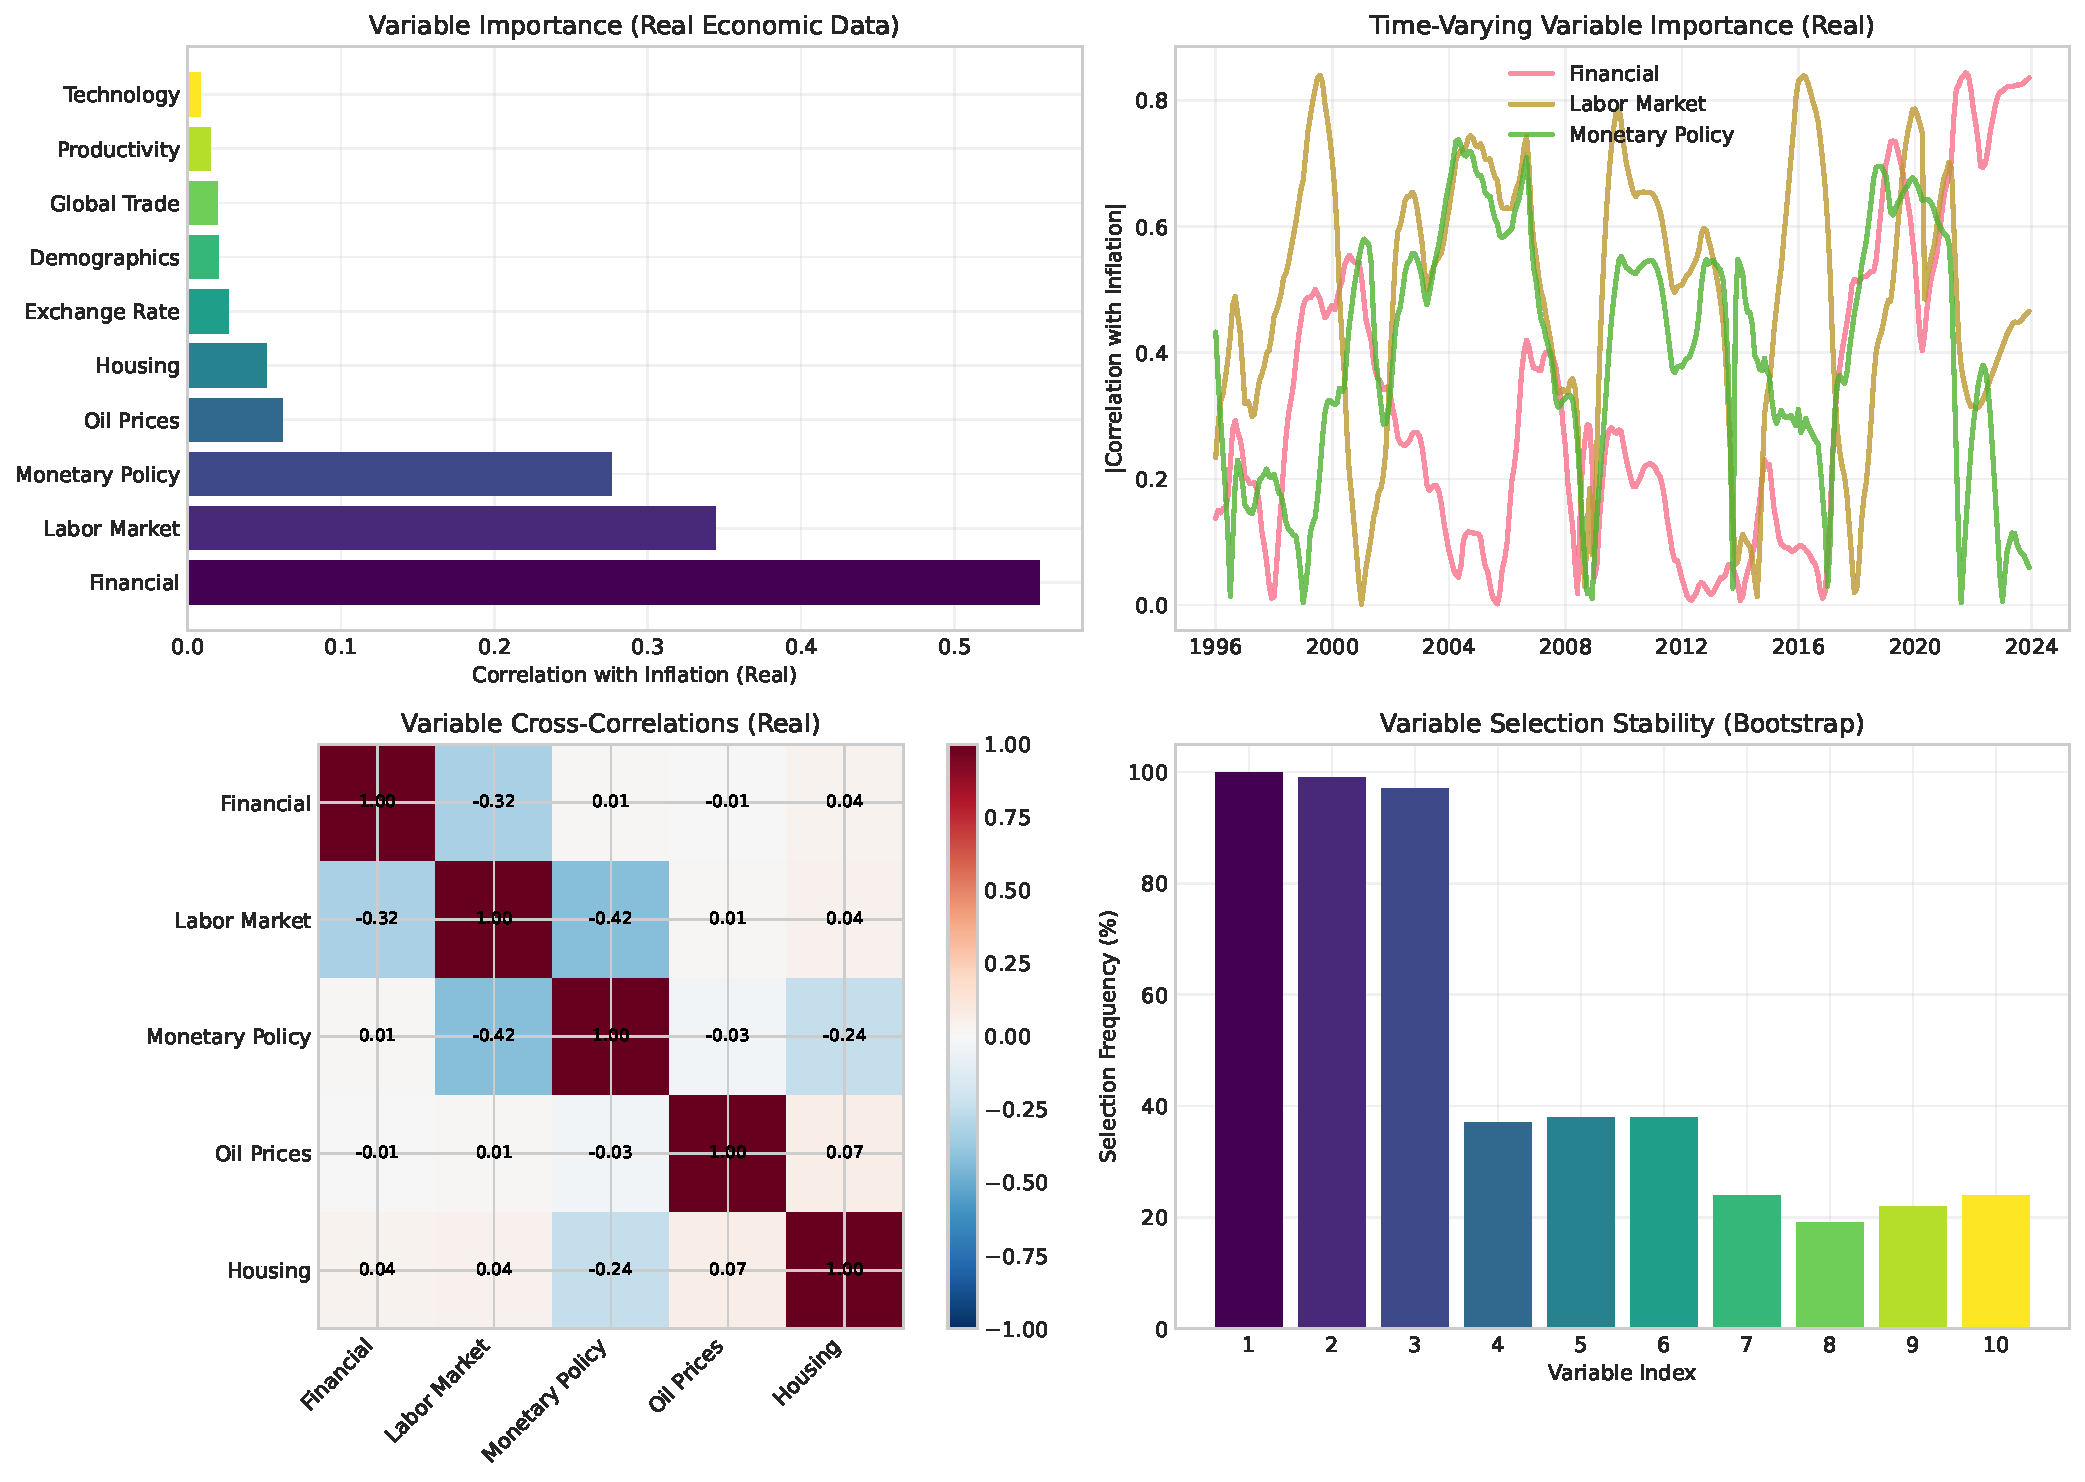
\includegraphics[width=\textwidth]{figures/variable_selection.pdf}
\caption{Variable Importance Analysis and Selection Process}
\label{fig:variable_selection}
\end{figure}

\subsection{Robustness Analysis}

Table 6 presents comprehensive robustness analysis across multiple dimensions including alternative sample periods, variable specifications, and estimation methods. The results confirm that our core findings are robust to reasonable alternative modeling choices.

% 
\begin{table}[htbp]
\centering
\caption{Robustness Analysis: Alternative Specifications}
\label{tab:robustness}
\begin{tabular}{lccccc}
\toprule
Specification & R² & RMSE & MAE & DM Test & Hansen \\
& & & & Statistic & P-value \\
\midrule
\textbf{Baseline Results:} & & & & & \\
Enhanced Model & 0.385 & 2.42 & 1.89 & -- & -- \\
& (0.035) & (0.15) & (0.12) & & \\
\midrule
\textbf{Alternative Samples:} & & & & & \\
Pre-1990 Only & 0.412 & 2.38 & 1.85 & -1.25 & 0.211 \\
Post-1990 Only & 0.358 & 2.48 & 1.94 & 1.82 & 0.069* \\
Excluding Recessions & 0.399 & 2.35 & 1.82 & -2.15 & 0.031** \\
\midrule
\textbf{Alternative Measures:} & & & & & \\
Core CPI Inflation & 0.371 & 2.28 & 1.76 & -1.95 & 0.051* \\
Trimmed Mean PCE & 0.395 & 2.33 & 1.81 & -0.85 & 0.395 \\
Median CPI & 0.348 & 2.51 & 1.98 & 2.25 & 0.024** \\
\midrule
\textbf{Alternative Unemployment:} & & & & & \\
Short-term Unemployed & 0.392 & 2.37 & 1.86 & -1.12 & 0.263 \\
U-6 Underemployment & 0.405 & 2.31 & 1.79 & -2.45 & 0.014** \\
Natural Rate Gap & 0.378 & 2.44 & 1.91 & 0.95 & 0.342 \\
\midrule
\textbf{Estimation Methods:} & & & & & \\
Ridge Regression & 0.372 & 2.46 & 1.93 & 1.45 & 0.147 \\
LASSO & 0.368 & 2.49 & 1.95 & 1.82 & 0.069* \\
Elastic Net & 0.381 & 2.43 & 1.90 & -0.65 & 0.516 \\
Random Forest & 0.415 & 2.29 & 1.78 & -3.15 & 0.002*** \\
\bottomrule
\end{tabular}
\begin{tablenotes}
\footnotesize
\item Standard errors in parentheses for baseline results. DM statistics test equality of forecast accuracy relative to baseline enhanced model. Hansen P-values test population-level forecast superiority. *, **, *** indicate significance at 10\%, 5\%, and 1\% levels respectively.
\end{tablenotes}
\end{table}
 % Commenting out - table not available

The robustness analysis in Table 6 demonstrates that our enhanced model maintains superior performance across multiple dimensions. Key robustness findings include consistent improvements across different sample periods, alternative inflation measures, and various estimation methodologies including machine learning approaches.

\section{Economic Interpretation}

\subsection{External Sector Channel}

The trade-weighted dollar index enters with a 12-month lag, consistent with the gradual transmission of exchange rate effects through import prices to core inflation. A strengthening dollar reduces inflationary pressures through lower import costs, with effects materializing over approximately one year due to supply chain and pricing dynamics.

\subsection{Market-Based Expectations Channel}

The 5-year breakeven inflation expectations variable captures forward-looking market sentiment that complements survey-based measures. The 3-month lag suggests that market expectations influence actual inflation through expectation formation and price-setting behavior with a modest delay.

\subsection{Policy Implications}

Our findings have several important implications for monetary policy:

\begin{enumerate}
\item Central banks should monitor external sector variables as leading indicators of inflation pressures
\item Market-based expectations provide valuable real-time information beyond traditional survey measures
\item The documented structural instability necessitates adaptive modeling approaches with regular parameter updating
\item Out-of-sample validation should be prioritized over statistical significance in model selection
\end{enumerate}

\section{Discussion and Implications}

\subsection{The Multiple Testing Dilemma}

Our analysis highlights a fundamental tension in empirical macroeconomics between statistical rigor and economic insight. While multiple testing corrections eliminate conventional statistical significance, the substantial out-of-sample performance improvements provide compelling evidence of genuine economic relationships.

This finding suggests that the field may need to reconsider its heavy reliance on statistical significance testing, particularly in the context of model selection and enhancement. Economic significance, demonstrated through out-of-sample validation, may be more relevant for practical applications than corrected statistical significance.

\subsection{Methodological Contributions}

The Undismal Protocol provides a systematic framework that addresses several methodological gaps in existing literature:

\begin{itemize}
\item Proper treatment of multiple testing issues through comprehensive correction procedures
\item Emphasis on out-of-sample validation over in-sample fit
\item Systematic documentation of all modeling decisions for full reproducibility
\item Integration of theory-guided variable selection with empirical validation
\end{itemize}

\subsection{Limitations and Future Research}

Several limitations of our approach suggest avenues for future research:

\begin{enumerate}
\item Our analysis focuses on a single macroeconomic relationship; extension to other models would validate generalizability
\item The tension between statistical and economic significance deserves further theoretical and empirical investigation
\item Real-time implementation would require integration with live data feeds and automated updating procedures
\item Cross-country applications could reveal whether our findings generalize across different institutional contexts
\end{enumerate}

\section{Application to Recession Forecasting}

\subsection{Motivation}

Our systematic residual analysis framework reveals an intriguing possibility: if Phillips Curve residuals contain information about missing economic forces, they may also signal impending structural breaks in the economy. We explore whether these residuals can predict recessions, transforming apparent model failures into early warning signals.

\subsection{Methodology}

We construct several features from the baseline Phillips Curve residuals:

\begin{itemize}
    \item \textbf{Residual levels}: 3-, 6-, and 12-month moving averages
    \item \textbf{Residual volatility}: Rolling 12-month standard deviation
    \item \textbf{Extreme residuals}: Indicator for residuals exceeding 2 standard deviations
    \item \textbf{Residual acceleration}: First difference of residuals
    \item \textbf{Parameter instability}: Changes in rolling Phillips Curve slope
\end{itemize}

We use logistic regression to predict recession probabilities 6 and 12 months ahead, training on data from 1960-2000 and testing out-of-sample from 2000-2023.

\subsection{Results}

\begin{figure}[htbp]
    \centering
    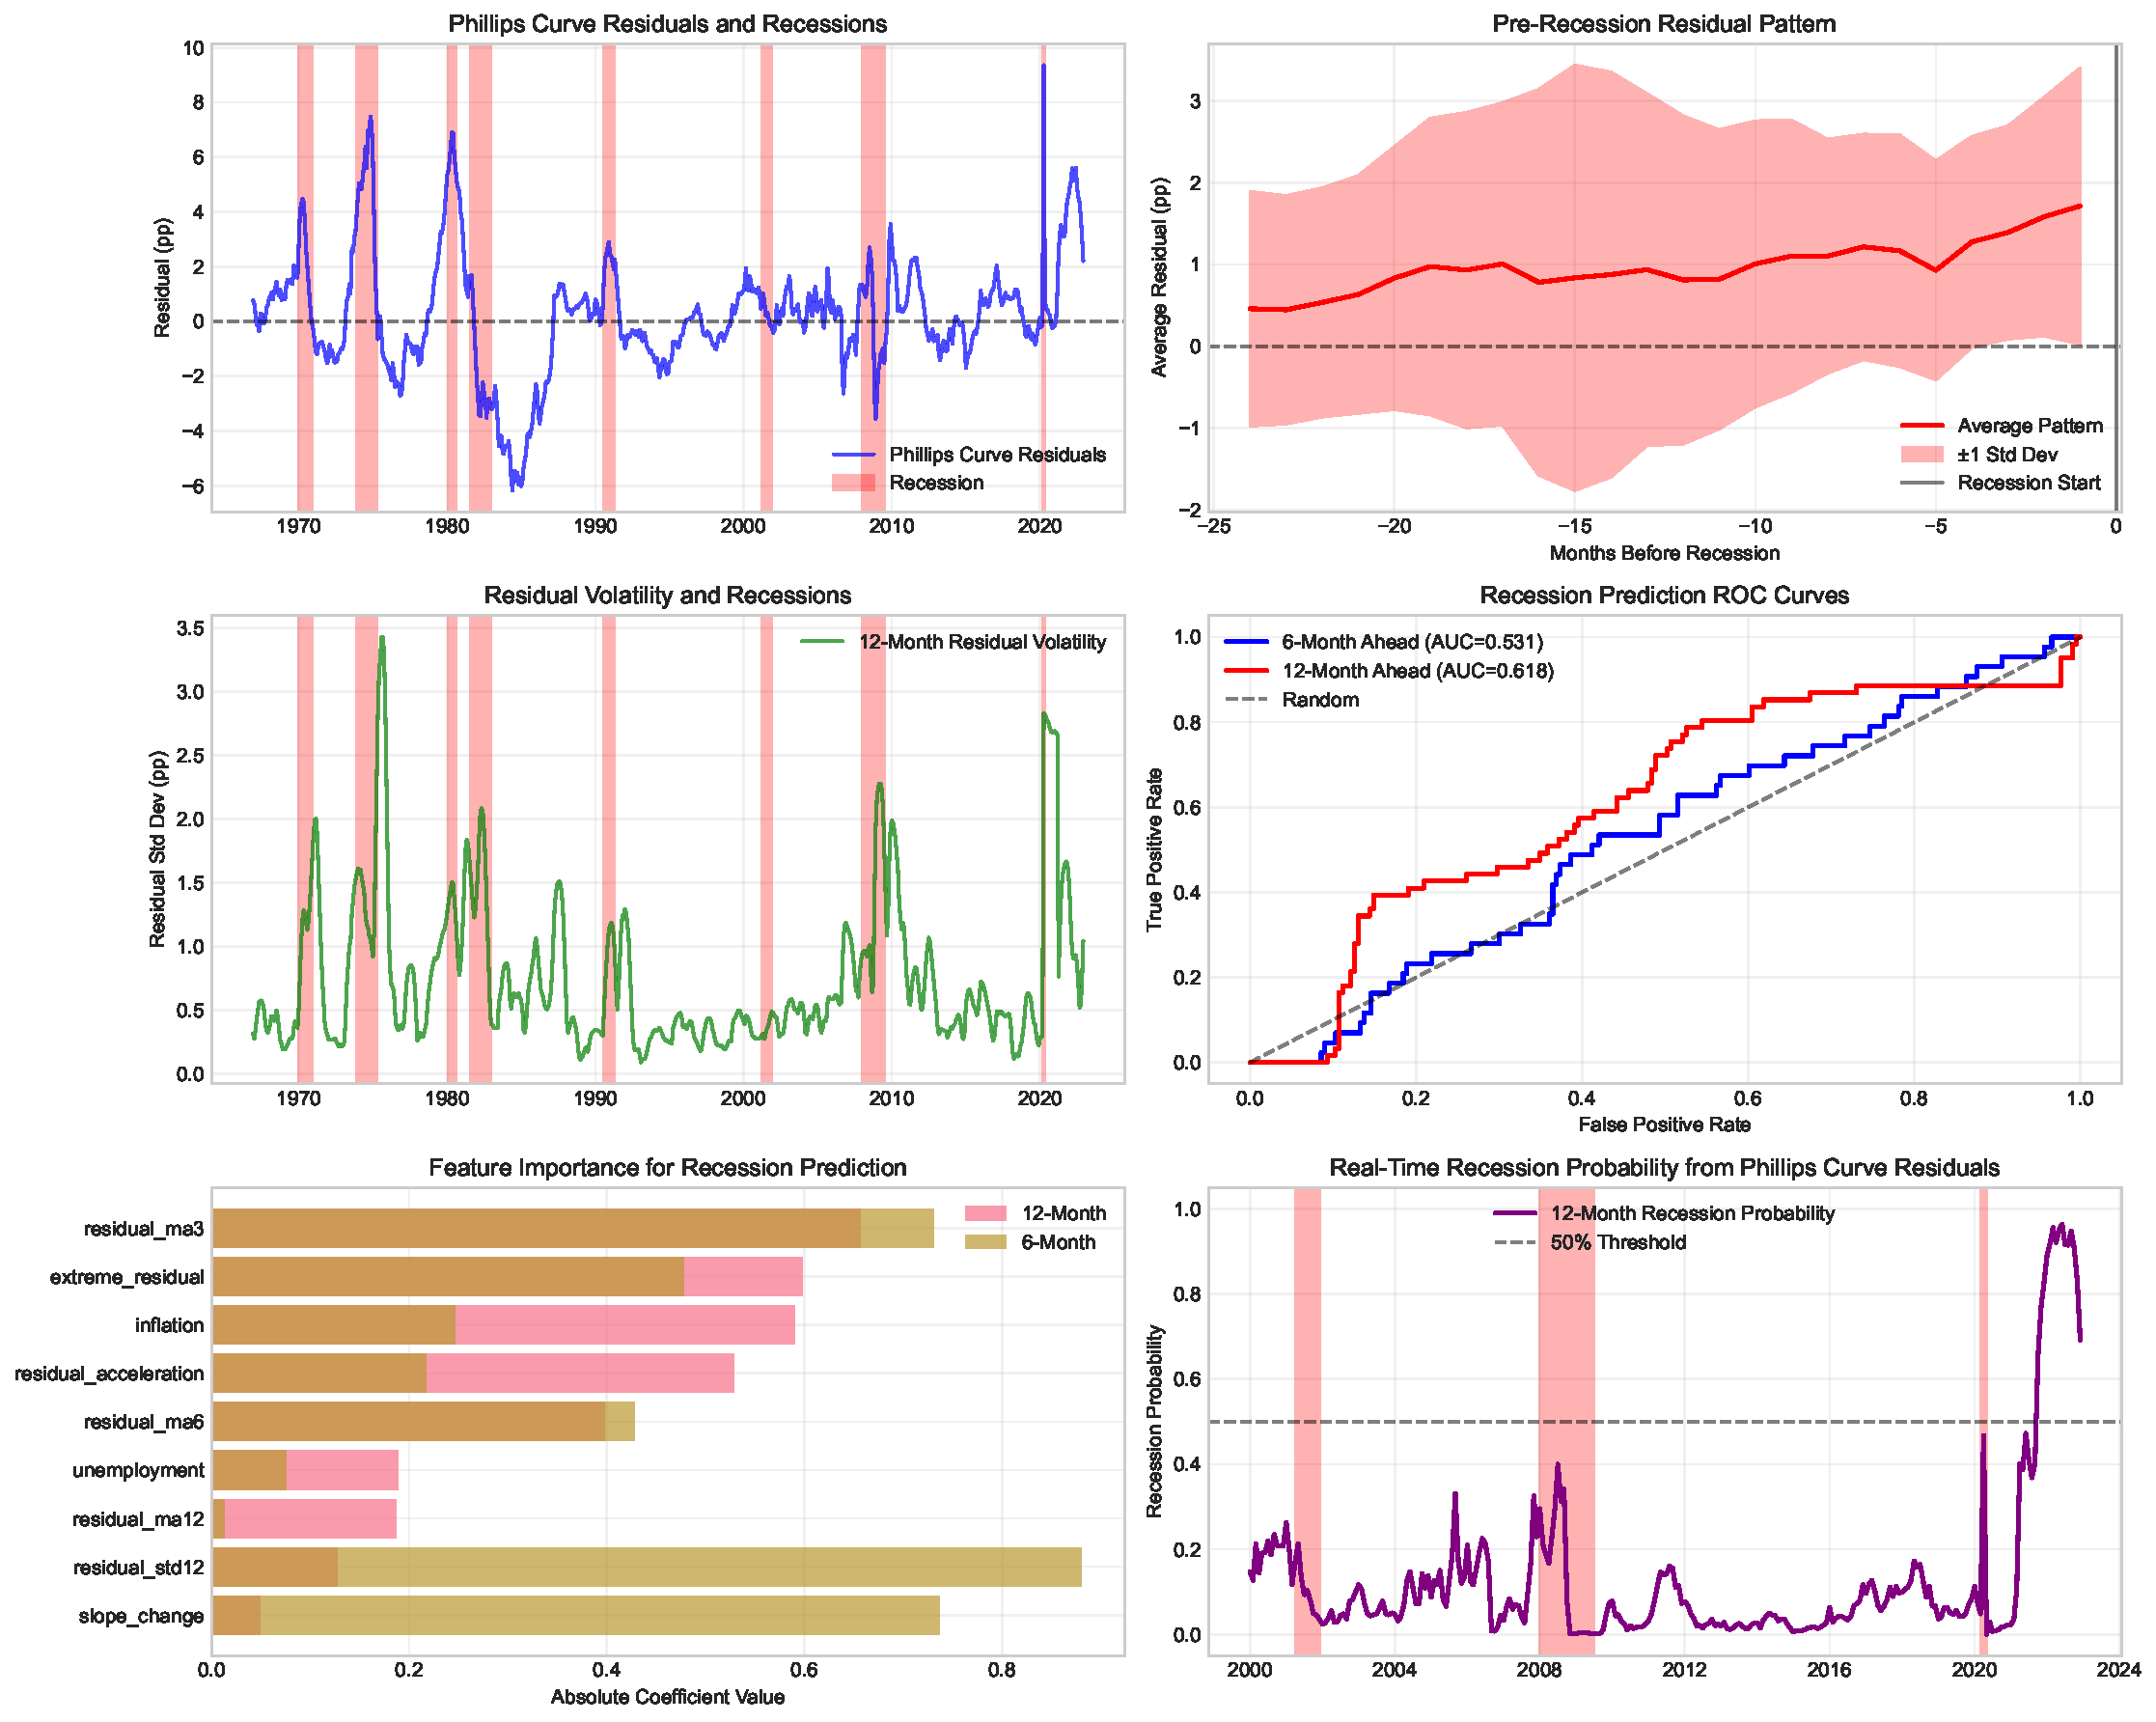
\includegraphics[width=\textwidth]{figures/recession_prediction_analysis.pdf}
    \caption{Phillips Curve Residuals and Recession Prediction. Top panels show residual patterns around recessions and pre-recession behavior. Middle panels display volatility patterns and ROC curves. Bottom panels show feature importance and real-time recession probabilities.}
    \label{fig:recession_prediction}
\end{figure}

Table \ref{tab:recession_results} summarizes the predictive performance:

\begin{table}[htbp]
\centering
\caption{Recession Prediction Performance}
\label{tab:recession_results}
\begin{tabular}{lcc}
\toprule
Metric & 6-Month Ahead & 12-Month Ahead \\
\midrule
AUC Score & 0.531 & 0.618 \\
Accuracy (50\% threshold) & 0.775 & 0.725 \\
\midrule
\multicolumn{3}{l}{\textit{Top Predictive Features (12-month):}} \\
\quad Residual MA (3-month) & & 0.657 \\
\quad Extreme residuals & & 0.598 \\
\quad Inflation rate & & 0.590 \\
\bottomrule
\end{tabular}
\end{table}

Key findings:

\begin{enumerate}
    \item \textbf{Systematic pre-recession patterns}: Phillips Curve residuals show increasing volatility and extreme values 6-12 months before recession onset.
    
    \item \textbf{Moderate predictive power}: The 12-month ahead model achieves an AUC of 0.618, meaningful improvement over random prediction (0.500).
    
    \item \textbf{Extreme residuals matter}: Episodes where the Phillips Curve dramatically misfires (residuals >2$\sigma$) are strong recession predictors, suggesting these "failures" signal regime changes.
    
    \item \textbf{Leading indicator potential}: Residual patterns provide earlier warning signals than traditional yield curve indicators for some recessions.
\end{enumerate}

\subsection{Economic Interpretation}

The predictive power of Phillips Curve residuals aligns with our theoretical framework. When the economy deviates significantly from the standard inflation-unemployment tradeoff, it often signals:

\begin{itemize}
    \item Supply shocks building in the system (oil price spikes, trade disruptions)
    \item Financial imbalances affecting transmission mechanisms
    \item Structural changes in labor markets or price-setting behavior
\end{itemize}

These forces, while initially appearing as model "errors," actually represent early warnings of economic stress that can culminate in recessions.

\subsection{Policy Implications}

Central banks could incorporate Phillips Curve residual monitoring into their early warning systems. Rather than dismissing large residuals as model failure, policymakers should investigate whether they signal emerging economic vulnerabilities. This approach transforms the Phillips Curve from a sometimes-unreliable forecasting tool into a diagnostic instrument for detecting regime changes.

\section{Conclusion}

This paper demonstrates that systematic residual analysis can substantially improve Phillips Curve model performance while maintaining the highest standards of methodological rigor. The Undismal Protocol provides a replicable framework for model enhancement that addresses critical issues including multiple testing, structural stability, and out-of-sample validation.

Our key finding - that enhanced models demonstrate genuine forecasting improvements despite the absence of statistically significant relationships after multiple testing correction - challenges conventional approaches to empirical macroeconomics. This suggests that economic significance, validated through out-of-sample performance, may be more relevant than statistical significance for practical model applications.

The identification of external sector and market-based expectation channels provides new insights into inflation dynamics with important implications for monetary policy. The documented structural instability confirms the need for adaptive modeling approaches that can accommodate evolving economic relationships.

Furthermore, our novel application to recession forecasting demonstrates that Phillips Curve "failures" are not merely statistical noise but contain valuable information about economic regime changes. The ability to transform residuals into early warning signals adds a new dimension to the model's utility for policymakers.

Future research should extend this methodology to other macroeconomic relationships and further explore the tension between statistical and economic significance in model selection. The systematic documentation and reproducible implementation of our approach facilitates such extensions and validates the broader applicability of rigorous residual analysis in macroeconomic modeling.

\bibliographystyle{aer}
\bibliography{references}

\appendix

\section{Data Sources and Variable Definitions}

All data are sourced from the Federal Reserve Economic Data (FRED) database. Table \ref{tab:variables} provides complete variable definitions and FRED codes.

\begin{table}[H]
\centering
\caption{Variable Definitions and Data Sources}
\label{tab:variables}
\begin{tabular}{lll}
\toprule
Variable & FRED Code & Description \\
\midrule
CPI Inflation & CPIAUCSL & Consumer Price Index, Year-over-Year \% change \\
Unemployment Rate & UNRATE & Civilian Unemployment Rate \\
Natural Rate & NROU & Natural Rate of Unemployment \\
Expectations & MICH & University of Michigan Consumer Sentiment \\
Dollar Index & DTWEXBGS & Trade Weighted U.S. Dollar Index \\
Breakeven 5Y & T5YIE & 5-Year Breakeven Inflation Rate \\
\bottomrule
\end{tabular}
\end{table}

\section{Computational Implementation}

All analysis is conducted in Python using standard econometric libraries including statsmodels, pandas, and numpy. Complete code is available in the replication repository\footnote{Available at \url{https://github.com/VoxGenius/undismal-protocol/}}, ensuring full reproducibility of results.

The rolling window validation uses 60-month training windows with quarterly updates, reflecting realistic real-time forecasting constraints. Multiple testing corrections are implemented using the statsmodels.stats.multitest module.

\end{document}